\documentclass[12pt]{../../vespers-sheet}
\usepackage{multicol}

\begin{document}

\chapter*{Vespers on Fridays in Eastertide\\ on Duplex Feasts}

\begin{center}
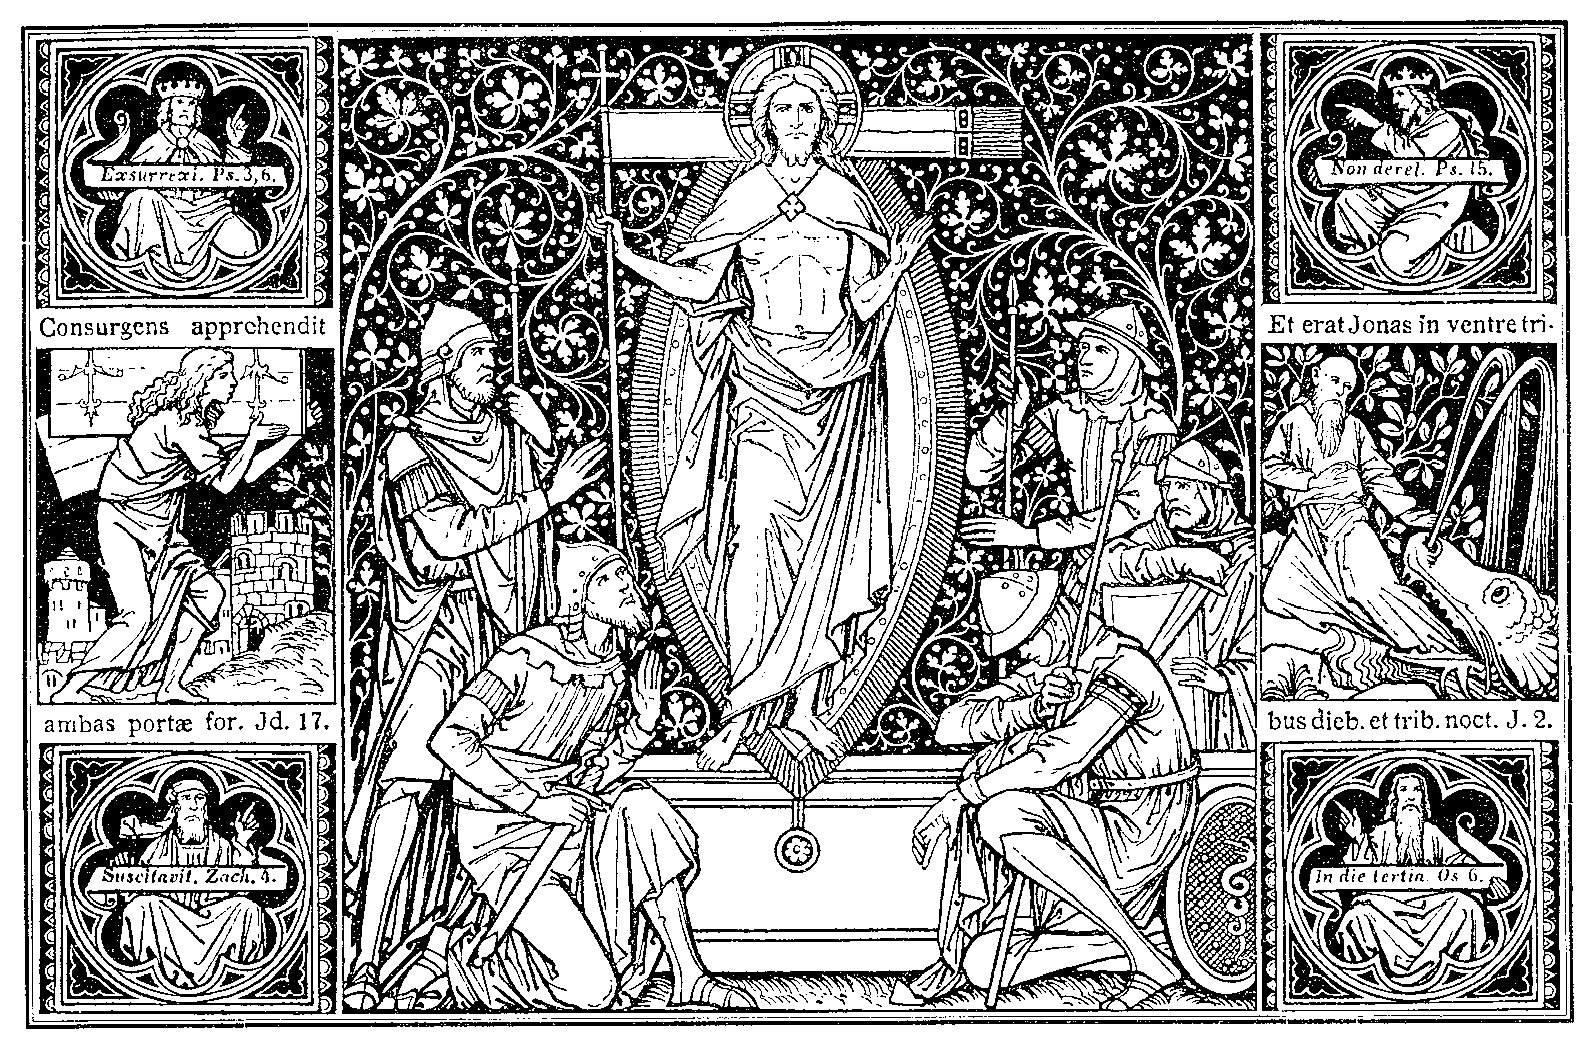
\includegraphics[width=\linewidth]{Resurrection.jpg}
\end{center}

\vfill\pagebreak

\begin{rubricbox}

{\color{red}When the leader kneels, all pray silently one \textit{Pater noster} (Our Father) and \textit{Ave Maria} (Hail Mary). All join the leader as he rises, and all make the sign of the cross with the leader as he intones:}

\end{rubricbox}

 \gresetinitiallines{1}
\gregorioscore{../../common/deus-in-adjutorium}

\textit{
O God, come to my assistance.
{\color{red}\Vbar.}~O Lord, make haste to help me.
Glory be to the Father, and to the Son, and to the Holy Spirit,
as it was in the beginning, is now, and ever shall be, world without end. Amen.
Alleluia. \textnormal{Or:} Praise to Thee, O Lord, King of endless glory.}

%\vfill\pagebreak

\section*{Psalm 139}

\textit{\textnormal{Ps.} Deliver me, O Lord, from the evil man: rescue me from the unjust man.}

\gresetinitiallines{0}
\gregorioscore{ps139-intonation}

 \begin{latinenglishsection}

\latinenglish{
	2. Qui cogitavérunt iniqui\textbf{tá}tes in \textbf{cor}de:~* tota die consti\textit{tu}\textit{é}\textit{bant} \textbf{pr\'{\ae}}lia.

3. Acuérunt linguas suas \textbf{sic}ut ser\textbf{pén}tis:~* venénum áspidum sub lá\textit{bi}\textit{is} \textit{e}\textbf{ó}rum.

4. Custódi me, Dómine, de manu \textbf{pec}ca\textbf{tó}ris:~* et ab homínibus iní\textit{quis} \textit{é}\textit{ri}\textbf{pe} me.

5. Qui cogitavérunt supplantáre \textbf{gres}sus \textbf{me}os:~* abscondérunt supérbi \textit{lá}\textit{que}\textit{um} \textbf{mi}hi:

6. Et funes exten\textbf{dé}runt in \textbf{lá}\textbf{que}um:~* juxta iter scándalum po\textit{su}\textit{é}\textit{runt} \textbf{mi}hi.

7. Dixi Dómino: Deus \textbf{me}us \textbf{es} tu:~* exáudi, Dómine, vocem depreca\textit{ti}\textit{ó}\textit{nis} \textbf{me}æ.

8. Dómine, Dómine, virtus sa\textbf{lú}tis \textbf{me}æ:~* obumbrásti super caput meum \textit{in} \textit{di}\textit{e} \textbf{bel}li.

9. Ne tradas me, Dómine, a desidério meo peccatóri:~{\color{red}\GreDagger} cogita\textbf{vé}runt \textbf{con}\textbf{tra} me,~* ne derelínquas me, ne for\textit{te} \textit{ex}\textit{al}\textbf{tén}tur.

10. Caput circúi\textbf{tus} e\textbf{ó}rum:~* labor labiórum ipsórum o\textit{pé}\textit{ri}\textit{et} \textbf{e}os.

11. Cadent super eos carbónes,~{\color{red}\GreDagger} in ignem de\textbf{jí}cies \textbf{e}os:~* in miséri\textit{is} \textit{non} \textit{sub}\textbf{sís}tent.

12. Vir linguósus non diri\textbf{gé}tur in \textbf{ter}ra:~* virum injústum mala cápi\textit{ent} \textit{in} \textit{in}\textbf{tér}itu.

13. Cognóvi quia fáciet Dóminus ju\textbf{dí}cium \textbf{ín}\textbf{o}pis:~* et \textit{vin}\textit{díc}\textit{tam} \textbf{páu}perum.

14. Verúmtamen justi confitebúntur \textbf{nó}mini \textbf{tu}o:~*{\color{red}\textit{(stand)}} et habitábunt recti \textit{cum} \textit{vul}\textit{tu} \textbf{tu}o.

15. {\color{red}\textit{(bow)}} Glória \textbf{Pa}tri, et \textbf{Fí}\textbf{li}o,~* et Spi\textit{rí}\textit{tu}\textit{i} \textbf{Sanc}to.

16. {\color{red}\textit{(rise)}} Sicut erat in princípio, et \textbf{nunc}, et \textbf{sem}per,~* et in s\'{\ae}cula sæ\textit{cu}\textit{ló}\textit{rum}. \textbf{A}men.	
}{
	2. Deliver me, O Lord, from the evil man: rescue me from the unjust man.

3. Who have devised iniquities in their hearts: all the day long they designed battles.

4. They have sharpened their tongues like a serpent: the venom of saps is under their lips.

5. Keep me, O Lord, from the hand of the wicked: and from unjust men deliver me. Who have proposed to supplant my steps.

6. The proud have hidden a net for me. And they have stretched out cords for a snare: they have laid for me a stumblingblock by the wayside.

7. I said to the Lord: Thou art my God: hear, O Lord, the voice of my supplication.

8. O Lord, Lord, the strength of my salvation: Thou hast overshadowed my head in the day of battle.

9. Give me not up, O Lord, from my desire to the wicked: they have plotted against me; do not Thou forsake me, lest they should triumph.

10. The head of them compassing me about: the labour of their lips shall overwhelm them.

11. Burning coals shall fall upon them; thou wilt cast them down into the fire: in miseries they shall not be able to stand.

12. A man full of tongue shall not be established in the earth: evil shall catch the unjust man unto destruction.

13. I know that the Lord will do justice to the needy, and will revenge the poor.

14. But as for the just, they shall give glory to Thy name: and the upright shall dwell with Thy countenance.

15. Glory be to the Father, and to the Son, and to the Holy Spirit.
 	
16. As it was in the beginning, is now, and ever shall be, world without end. Amen.
}

\end{latinenglishsection}

\section*{Psalm 140}

\textit{\textnormal{Ps.} I have cried to Thee, O Lord: hear me: hearken to my voice, when I cry to Thee.}

\gresetinitiallines{0}
\gregorioscore{ps140-intonation}

 \begin{latinenglishsection}

\latinenglish{
	2. Dirigátur orátio mea sicut incénsum in con\textbf{spéc}tu \textbf{tu}o:~* elevátio mánuum meárum sacrifíci\textit{um} \textit{ves}\textit{per}\textbf{tí}num.

3. Pone, Dómine, custódiam \textbf{o}ri \textbf{me}o:~* et óstium circumstántiæ \textit{lá}\textit{bi}\textit{is} \textbf{me}is.

4. Non declínes cor meum in \textbf{ver}ba ma\textbf{lí}\textbf{ti}æ:~* ad excusándas excusatió\textit{nes} \textit{in} \textit{pec}\textbf{cá}tis.

5. Cum homínibus operántibus in\textbf{i}qui\textbf{tá}tem:~* et non communicábo cum e\textit{léc}\textit{tis} \textit{e}\textbf{ó}rum.

6. Corrípiet me justus in misericórdia, et \textbf{in}cre\textbf{pá}\textbf{bit} me:~* óleum autem peccatóris non impín\textit{guet} \textit{ca}\textit{put} \textbf{me}um.

7. Quóniam adhuc et orátio mea in\\ benepláci\textbf{tis} e\textbf{ó}rum:~* absórpti sunt juncti petræ jú\textit{di}\textit{ces} \textit{e}\textbf{ó}rum.

8. Audient verba mea quóniam \textbf{pot}u\textbf{é}runt:~* sicut crassitúdo terræ erúpta \textit{est} \textit{su}\textit{per} \textbf{ter}ram.

9. Dissipáta sunt ossa nostra secus inférnum:~{\color{red}\GreDagger} quia ad te, Dómine, Dómine, \textbf{ó}culi \textbf{me}i:~* in te sperávi, non áuferas \textit{á}\textit{ni}\textit{mam} \textbf{me}am.

10. Custódi me a láqueo, quem statu\textbf{é}runt \textbf{mi}hi:~* et a scándalis operántium \textit{in}\textit{i}\textit{qui}\textbf{tá}tem.

11. Cadent in retiáculo ejus \textbf{pec}ca\textbf{tó}res:~*\\ singuláriter sum e\textit{go} \textit{do}\textit{nec} \textbf{tráns}eam.

12. {\color{red}\textit{(bow while seated)}} Glória \textbf{Pa}tri, et \textbf{Fí}\textbf{li}o,~* et Spi\textit{rí}\textit{tu}\textit{i} \textbf{Sanc}to.

13. {\color{red}\textit{(rise, remaining seated)}} Sicut erat in princípio, et \textbf{nunc}, et \textbf{sem}per,~* et in s\'{\ae}cula sæ\textit{cu}\textit{ló}\textit{rum}. \textbf{A}men.	
}{
	2. Let my prayer be directed as incense in thy sight; the lifting up of my hands, as evening sacrifice.
	
3. Set a watch, O Lord, before my mouth: and a door round about my lips.

4. Incline not my heart to evil words; to make excuses in sins. 

5. With men that work iniquity: and I will not communicate with the choicest of them.

6. The just shall correct me in mercy, and shall reprove me: but let not the oil of the sinner fatten my head. 

7. For my prayer also shall still be against the things with which they are well pleased: Their judges falling upon the rock have been swallowed up. 

8. They shall hear my words, for they have prevailed: As when the thickness of the earth is broken up upon the ground: 

9. Our bones are scattered by the side of Hell. But o to thee, O Lord, Lord, are my eyes: in thee have I put my trust, take not away my soul.

10. Keep me from the snare, which they have laid for me, and from the stumbling blocks of them that work iniquity.

11. The wicked shall fall in his net: I am alone until I pass.

12. Glory be to the Father, and to the Son, and to the Holy Spirit.
 	
13. As it was in the beginning, is now, and ever shall be, world without end. Amen.
}

\end{latinenglishsection}

\section*{Psalm 141}

\textit{\textnormal{Ps.} I cried to the Lord with my voice: with my voice I made supplication to the Lord.}

\gresetinitiallines{0}
\gregorioscore{ps141-intonation}

 \begin{latinenglishsection}

\latinenglish{
	2. Effúndo in conspéctu ejus orati\textbf{ó}nem \textbf{me}am,~* et tribulatiónem meam ante \textit{ip}\textit{sum} \textit{pro}\textbf{nún}tio.

3. In deficiéndo ex me \textbf{spí}ritum \textbf{me}um:~* et tu cognovísti \textit{sé}\textit{mi}\textit{tas} \textbf{me}as.

4. In via hac, qua \textbf{am}bu\textbf{lá}bam,~* abscondérunt \textit{lá}\textit{que}\textit{um} \textbf{mi}hi.

5. Considerábam ad déxteram, \textbf{et} vi\textbf{dé}bam:~* et non erat qui \textit{co}\textit{gnó}\textit{sce}\textbf{ret} me.

6. Périit \textbf{fu}ga \textbf{a} me:~* et non est qui requírat \textit{á}\textit{ni}\textit{mam} \textbf{me}am.

7. Clamávi ad te, Dómine,~{\color{red}\GreDagger} dixi: Tu \textbf{es} spes \textbf{me}a,~* pórtio mea in \textit{ter}\textit{ra} \textit{vi}\textbf{vén}tium.

8. Inténde ad deprecati\textbf{ó}nem \textbf{me}am:~* quia humili\textit{á}\textit{tus} \textit{sum} \textbf{ni}mis.

9. Líbera me a perse\textbf{quén}ti\textbf{bus} me:~* quia confor\textit{tá}\textit{ti} \textit{sunt} \textbf{su}per me.

10. Educ de custódia ánimam meam ad confiténdum \textbf{nó}mini \textbf{tu}o:~*\\ me exspéctant justi, donec re\textit{trí}\textit{bu}\textit{as} \textbf{mi}hi.

11. {\color{red}\textit{(bow while seated)}} Glória \textbf{Pa}tri, et \textbf{Fí}\textbf{li}o,~* et Spi\textit{rí}\textit{tu}\textit{i} \textbf{Sanc}to.

12. {\color{red}\textit{(rise, remaining seated)}} Sicut erat in princípio, et \textbf{nunc}, et \textbf{sem}per,~* et in s\'{\ae}cula sæ\textit{cu}\textit{ló}\textit{rum}. \textbf{A}men.	
}{
	2. In his sight I pour out my prayer, and before him I declare my trouble:
	
3. When my spirit failed me, then thou newest my paths. 

4. In this way wherein I walked, they have hidden a snare for me.

5. I looked on my right hand, and beheld, and there was no one that would know me. 

6. Flight hath failed me: and there is no one that hath regard to my soul.

7. I cried to thee, O Lord: I said: Thou art my hope, my portion in the land of the living.

8. Attend to my supplication: for I am brought very low. 

9. Deliver me from my persecutors; for they are stronger than I.

10. Bring my soul out of prison, that I may praise thy name: the just wait for me, until thou reward me.

11. Glory be to the Father, and to the Son, and to the Holy Spirit.
 	
12. As it was in the beginning, is now, and ever shall be, world without end. Amen.
}

\end{latinenglishsection}

%{\color{red}\textit{All chant the Alleluia antiphon together:}}

\gresetinitiallines{0}
\gregorioscore{pss-antiphon}
%\textit{\textnormal{Ant.} Alleluia, alleluia, alleluia.}


\begin{rubricbox}

{\color{red}Continue to the insert for the day for the Little Chapter, Hymn, Magnificat, Collect, any Commemorations, and the Conclusion.}

\end{rubricbox}

\end{document}